\documentclass[12pt,oneside]{fithesis2}

% ===== LOADING PACKAGES =====
% language settings, main documnet language last
\usepackage[english]{babel}
% enabling new fonts support (nicer)
\usepackage{lmodern}
% setting input encoding
\usepackage[utf8]{inputenc}
% setting output encoding
\usepackage[T1]{fontenc}
% fithesis2 requires csquotes
\usepackage{csquotes}
% set page margins
\usepackage[top=3.5cm, bottom=3cm, left=2.4cm, right=2.4cm]{geometry}
% package to make bullet list nicer
\usepackage{enumitem}
% math symbols and environments
\usepackage{mathtools}
% packages for complex tables
\usepackage{tabularx}
\usepackage{multirow}
\usepackage{siunitx}
\usepackage{dcolumn}
\usepackage{array}
% enable page rotation
\usepackage{pdflscape}
% bibliography management
\usepackage[backend=biber, 		% use biber as backend instead of BiBTeX
	bibstyle=ieee-alphabetic, 	% bibliography style: IEEE with alphabetic citations
	citestyle=alphabetic, 		% citation style
	url=true, 					% display urls in bibliography
	hyperref=auto,				% detect hyperref and create links
	block=ragged 				% format bibliography into blocks, ragged on right
]{biblatex}
\addbibresource{thesis.bib}
% generating hyperlinks in document
\usepackage{url}
\usepackage[plainpages=false,pdfpagelabels,colorlinks=true]{hyperref}

% ===== MAIN DOCUMENT SETTINGS =====
% adjusting hyphenation penalties
\tolerance=10000
\hyphenpenalty=500
% space between paragraphs
\setlength{\parskip}{0.6em plus0.2em minus0.2em}
% set smaller default spacing in itemize
%\setitemize{itemsep=0.2em,topsep=0pt,parsep=0pt,partopsep=0pt}
% set default itemize symbol to square
\newcommand{\squarebullet}{\textcolor{black}{\raisebox{0.15em}{\rule{4pt}{4pt}}}}
%\renewcommand{\labelitemi}{\squarebullet}
%\renewcommand{\labelitemi}{\scriptsize$\blacksquare$} 
\newenvironment{myItemize}{
  \begin{itemize}[leftmargin=2em,rightmargin=1em,itemsep=\parskip ,parsep=0em,topsep=0em,partopsep=0em]
%  \setlength{}{2em}
%  \setlength{\rightmargin}{1.5em}
%  \setlength{\itemsep}{0.2em}
%  \setlength{\parsep}{0em}
%  \setlength{\topsep}{0em}
%  \setlength{\partopsep}{0em}
%  \setlength{\parskip}{0em}
  \renewcommand{\labelitemi}{\squarebullet}
  \renewcommand{\labelitemii}{$\diamond$}
}{
  \end{itemize}
}
% FI THESIS settings
\thesistitle{Usage of evolvable circuit \\for statistical testing \\of randomness}
\thesissubtitle{Bachelor thesis}
\thesisstudent{Martin Ukrop}
\thesiswoman{false}
\thesisfaculty{fi}
\thesisyear{spring 2013}
\thesisadvisor{RNDr.\ Petr Švenda,\ Ph.D.}
\thesislang{en}

% ===== NEW COMMANDS (TABLES) =====
% verrical centering in 2 row cell
\newcommand{\m}[1]{\multirow{2}*{#1}}
% rotated (one or multi line) table cell
\newcommand{\rotatedHeader}[2][l]{\rotatebox{90}{\begin{tabular}[#1]{@{}l}#2\end{tabular}}}
% results table for eStream
\newcommand{\resultsTableEstream}[1]{%
\newcolumntype{C}{>{\centering\arraybackslash}X}%
\begin{tabularx}{\textwidth}{|r*{3}{||S[table-format=2.1]|S[table-format=3.0]|C}|} \hline
\multirow{1}*{\raisebox{-\height-0.3cm}{\rotatebox{90}{\# of rounds}}} & \multicolumn{9}{c|}{IV and key reinitialization} \\ \cline{2-10}
& \multicolumn{3}{c||}{once for run} & 
\multicolumn{3}{c||}{for each test set} & 
\multicolumn{3}{c|}{for each test vector} \\ \cline{2-10}
& \multicolumn{1}{c|}{\rotatedHeader{Dieharder\\(x/20)}} & \multicolumn{1}{c|}{\rotatedHeader{\textsc{Sts Nist}\\(x/162)}} &  \rotatedHeader{EACirc\\(\textsc{aam})}
& \multicolumn{1}{c|}{\rotatedHeader{Dieharder\\(x/20)}} & \multicolumn{1}{c|}{\rotatedHeader{\textsc{Sts Nist}\\(x/162)}} & \rotatedHeader{EACirc\\(\textsc{aam})}
& \multicolumn{1}{c|}{\rotatedHeader{Dieharder\\(x/20)}} & \multicolumn{1}{c|}{\rotatedHeader{\textsc{Sts Nist}\\(x/162)}} & \rotatedHeader{EACirc\\(\textsc{aam})} \\ \hline \hline
#1
\end{tabularx}}
% results table for SHA-3
\newcommand{\resultsTableSha}[1]{%
\newcolumntype{C}{>{\centering\arraybackslash}X}%
\begin{tabularx}{7.2cm}{|r||S[table-format=2.1]|S[table-format=3.0]|C|} \hline
\raisebox{0cm}{\rotatebox{90}{\# of rounds }} & 
\multicolumn{1}{c|}{\rotatedHeader{Dieharder\\(x/20)}} & 
\multicolumn{1}{c|}{\rotatedHeader{\textsc{Sts Nist}\\(x/162)}} & 
\rotatedHeader{EACirc\\(\textsc{aam})} \\ \hline \hline
#1
\end{tabularx}}
% two column part
\newcommand{\twoColumns}[2]{%
\begin{minipage}{0.47\textwidth}
\centering
#1
\end{minipage}
\hfill
\begin{minipage}{0.47\textwidth}
\centering
#2
\end{minipage}
}

% ===== BEGIN DOCUMENT =====
\begin{document}

\FrontMatter
\ThesisTitlePage

\begin{ThesisDeclaration}
\DeclarationText
\AdvisorName
\end{ThesisDeclaration}

\begin{ThesisThanks}
I'd like to thank Petr for his guidance, enthusiasm and inspiring discussions.
I also owe much to my mom and brother for their continuous support. Thank you.

\noindent
Further thanks goes to all my friends that had to put up with my enthusiasm 
and numerous details of the research they never asked for $\ddot\smile$.

\noindent
Last but not least, I'd like to acknowledge the Laboratory of Security and Applied Cryptography and 
the National Grid Infrastructure MetaCentrum for providing access to their computing and storage facilities.
\end{ThesisThanks}

\begin{ThesisAbstract}
This thesis explores automated methods of creating statistical randomness tests. Tests are created as hardware-like circuits using
EACirc, framework for automatic problem solving based on genetic programming. The improvements and current capabilities
of the framework are described along with a set of reference experiments.
The framework is then used to assess the randomness of outputs produced by chosen eStream cipher candidates
and SHA-3 hash function candidates.
The success of tests generated by EACirc is compared to standard statistical batteries (Dieharder, STS NIST).
\end{ThesisAbstract}

\begin{ThesisKeyWords}
statistical randomness, random distinguisher, evolutionary algorithms, genetic programming, software circuit, 
hash function, SHA-3, stream ciphers, eStream
\end{ThesisKeyWords}

\MainMatter
\tableofcontents
\chapter{Introduction}
\label{chap:intro}



\begin{myItemize}
\item problem description
\item motivation -> EACirc
\item summary of experiments to follow
\item we = team of EACirc
\item work and research done by me, if not stated otherwise (but consulted within the team!)
\item licence of EACirc, licence of thesis text
\item fithesis2 used
\end{myItemize}

\chapter{Statistical randomness testing}
\label{chap:stat-rand-testing}

The goal of randomness testing is to determine, whether the data provided is \textit{random}. 
The problem comes with the definition of randomness, since in truly random data, 
each fixed subsequence (e.\,g.\ sequence of a hundred zeroes) has the same probability of appearing.
Thus, statistical metrics have been developed to asses the matter of randomness.

All the statistical randomness tests are based on mathematical properties that hold for
\textit{most} of the random sequences with a sufficient length.
A simple example of such a property states that in each binary sequence the number of ones and zeroes should be 
approximately the same. It is crucial to be aware, that this will not hold for \textit{all} sequences (see the example above),
but the probability of randomly generating such a sequence sharply decreases with the increasing length.

Paragraph summarising statistical batteries \autoref{fig:workflow-statistical-batteries}.

\begin{figure}[b!]
\centering
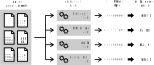
\includegraphics[width=\textwidth]{images/workflow-statistical-batteries}
\caption{Simplified work-flow of statistical batteries such as STS NIST or Dieharder.}
\label{fig:workflow-statistical-batteries}
\end{figure}

Randomness testing based on statistical properties of data has both drawbacks and benefits, main of which are discussed below.
\begin{myItemize}
\item \textbf{Speed}\\
Once the tests are implemented, they do not require excessive amount of time to perform -- 
the data is usually processed just once in a linear fashion.
\item \textbf{Universality}\\
Statistical tests can by applied to any binary data regardless of its origin -- they perform equally well. 
This can be viewed both as an advantage and disadvantage, since tests cannot be effortlessly adapted to specific situations.
\item \textbf{One-way design}\\
The creation of new test must be preceded by the idea and analysis of some useful statistical property. This part may be 
very complicated and usually requires extensive mathematical skills.
\item \textbf{Results interpretation}\\
The ever-present ambiguity in statistical measurements sometimes makes the results interpretation a highly non-trivial task.
It is crucial to understand what do the results indicate and what they do not. The above-mentioned finite sequence of binary zeroes
fails most of the statistical randomness tests, but its generation is just as probable 
as any other fixed binary sequence of the same length.
Put in another words, even the true random generator must produce non-random looking sequences once in a while.
\end{myItemize}

\noindent
In practise, statistical randomness testing is being widely used in fields where the quality of random data is crucial, 
such as cryptography. To ease the assessment process, several statistical randomness testing suites have been developed, 
some of which are discussed below.

\section{Statistical Test Suite by NIST}
\label{sec:sts-nist}

Perhaps the most widely used battery of statistical tests is the Statistical Testing Suite 
by National Institute of Standards and Technology (STS NIST).
The primary motivations for developing this test suite was the need of standardised tests for detecting non-randomness 
in binary (pseudo-)random sequences utilized in cryptographic applications. As well as designing the tests,
NIST provides their reference implementation and guidance in their use and application. \parencite{sts-nist}

The battery consists of 15 different tests, some of which can be run with several parameters. 
For detailed description of the tests, see the original documentation \parencite{sts-nist-documentation}. 
The implementation provided by NIST supports variable input data length and arbitrary number of independent data streams. 
The testing results provide the combined p-value of all data streams and the number of passed runs for each test 
according to the set significance level. 
Detailed setting used for the purposes of this thesis can be found in \autoref{sec:settings-statistics}.

\section{Diehard battery of tests}
\label{sec:diehard}

The second (unofficial) standard of statistical randomness testing is the Diehard Battery of Tests of Randomness, 
developed by George Marsaglia over several years at Florida State University. \parencite{diehard} 
Although now becoming slightly outdated, they were one of the first and most-well known 
in the pioneering years of statistical testing of randomness. 
For long, the Diehard Battery of Tests was considered a golden standard along with STS NIST.

The battery consist of 12 different tests. The original implementation, documentation and test descriptions are still available,
but since the code has not been revised from its creation in 1995, we chose not to use Marsaglia's original implementation.

\section{Dieharder: A Random Number Test Suite}
\label{sec:dieharder}

Dieharder, as its predecessors, aims to ease the testing of (pseudo-)random generators and data for a variety purposes in research 
and cryptography. Developed by Robert G. Brown at the Duke University, it is designed to be as extensible as possible, 
allowing easy implementation of new tests and generators for testing. Most of the tests used allow for 
modifying the default parameters, enabling advanced users to fine-tune the testing process.
According to its creators, it is intended to be the ``Swiss army knife of random number test suite'', 
or if you prefer, ``the last suite you'll ever ware'' for testing random numbers. \parencite{dieharder}

After designing the testing framework, the development team gradually reimplemented and improved the original tests from 
the Diehard Battery of Tests of Randomness (see \autoref{sec:diehard}), 
the tests from STS NIST (see \autoref{sec:sts-nist}) and began to prepare and implement their own new tests.
The suite now contains 31 different tests from various sources. Tests can be run selectively.
The testing results provide the combined p-value for each test and a verdict of \textsc{passed}, \textsc{weak} or \textsc{failed}
according to the set significance levels.
Detailed settings used for the purposes of this thesis can be found in \autoref{sec:settings-statistics}.

\section{Drawbacks of human-designed statistical tests}
\label{sec:limits-stat-testing}

Although convenient in some ways, statistical randomness testing based on human-designed tests has several important drawbacks.
As mentioned above, the test creation must be preceded by an idea of mathematical property and its thorough analysis, 
which can be extremely time- and people-consuming. Further on, the tests are limited to one particular property and
adapting them to specific situation requires beginning the process of test creation all over again.

Both of the above-mentioned problems would be resolved if tests of comparable quality could be generated automatically, without 
the help of human specialists. Such concept and its comparison with human-generated tests is presented in the following chapters.

\chapter{Evolution-based randomness testing}
\label{chap:evo-based-testing}

In this chapter we try to describe a method of automatically generating statistical randomness tests. Compared to the standard
(manual) way of their creation, our approach would have a couple of advantages: 
\begin{myItemize}
\item no prior knowledge of statistical properties of random data is needed;
\item test creation does not require excessive human analytical labour;
\item tests adapted for specific situations can be easily developed;
\item atypical and/or yet unknown data properties may be used.
\end{myItemize}

\noindent
The main idea is to use supervised learning techniques based on evolutionary algorithms to design and further 
optimize a successful \textit{distinguisher} -- the test determining whether its input comes from a truly random source or not. 
The distinguisher will be represented as a hardware-like circuit consisting of a number of interconnected simple functions.
The evolution will use the principles of genetic programming.

\section{Basic principles of genetic programming}
\label{sec:basic-ga}

Genetic programming \parencite{genetic-programming} is a biologically inspired supervised learning technique. 
It tries to converge to optimal 
solution by making subtle changes to previous partial solutions, assessing their impact and propagating the perspective changes
until reaching the desired success rate. The existence of partial problem solutions is therefore essential.
The main flow of evolution implemented by genetic programming is as follows:
\begin{enumerate} \rightskip=2em
\item Firstly, a random set of partial solutions is generated. The solutions may be highly unsuccessful,
but some will nonetheless be better than others. This set of solutions is called a \textit{population}.
\item Secondly, the success of all individual solutions from the population is evaluated. The assessment is done using
a so called \textit{fitness function}. The quality of this function is crucial to the whole algorithm, as it
distinguishes the better and more successful partial solutions from the worse ones.
\item A new population of solutions is created by making a \textit{sexual crossover} of the best solutions from the 
previous generation. Informally put, solutions are subject to the survival of the fittest.
\item A small random change may be applied to some individuals in the new population. This \textit{mutation} prevents
the population from getting stuck in the local optimum and increases the chances of reaching a global optimum.
\item Steps 2-4 are iterated over and over, until the desired success rate of the population is achieved or the
required number of generations have evolved.
\end{enumerate}

\noindent
The principles of evolutionary algorithms induce a couple of design limitations and disadvantages. 
The most important ones include:
\begin{myItemize}
\item Only problems with a sufficient space of partial solutions are applicable, since the individuals must be assessed 
to determine the fittest.
\item A small change in the solution should induce only a small change in the individual's fitness. If the changes were
too rapid, the evolution wouldn't be able to stabilize on the better and more successful solutions.
\item The evolution phase can be computationally very expensive, since making only small improvements to the individuals may require
high number of generations evolved.
\item It may be quite difficult to fine-tune the parameters (such as population size, mutation and crossover probabilities)
to achieve the best results.
\end{myItemize}

\noindent
To counterweight the drawbacks, it must be noted, that evolutionary algorithms allow us to create solution not just for particular
instance of the problem, but to the whole set of similar problems -- we may be trying to evolve a universal solver, 
rather than for the solution itself. 
This improves the computation complexity, because after an expensive learning phase, the evolved solver may be used
repeatedly on multiple instances of the problem. However, the evolution of the general solver can be trickier than it seems,
since over-learning (i.\,e. finding the solution just to the particular instance of the problem) has to be avoided.

\section{Using software-emulated circuits}
\label{sec:sw-circuits}

Our goal is to create a simple circuit performing the desired task -- distinguishing the random and non-random data streams.
Thus, let's consider solutions in the form of of a hardware-like circuits with gates (\textit{function nodes}) 
and a set of wires (\textit{node connectors}).
Each node is responsible for computation of a simple function on its inputs (e.\,g.\ binary \textsc{and} operation).
Circuit nodes are positioned into layers, where outputs from one layer are connected to inputs of the next. Input of the whole
circuit is used as an input for the first layer and output of the last layer is considered the output of the entire circuit.
Connectors may only link adjacent layers, but may cross each other (contrary to real single-layer hardware circuits).
An example of such hardware-like circuit can be seen in \autoref{fig:circuit-example}.

\begin{figure}[t!]
\centering
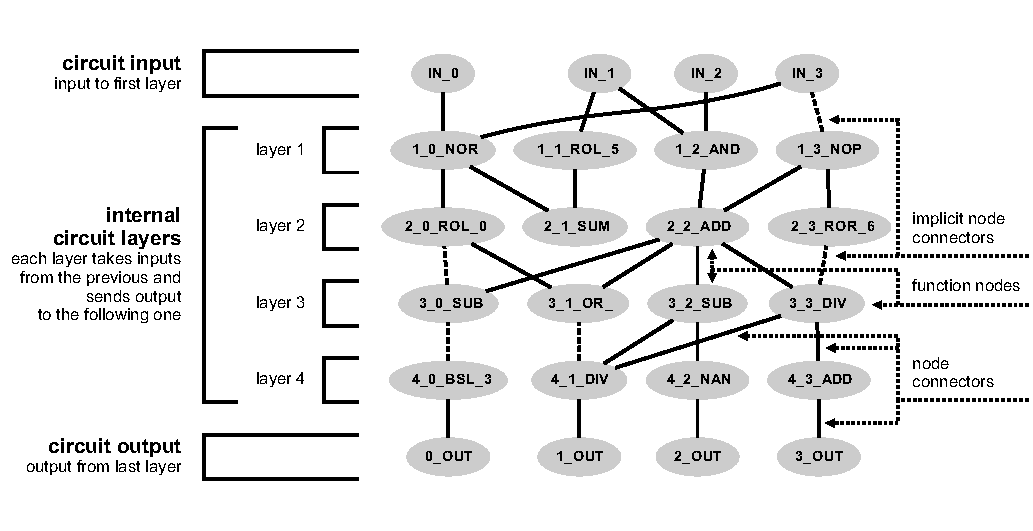
\includegraphics[width=\textwidth]{images/circuit-final}
\caption{Simple example of software-emulated circuit.}
\label{fig:circuit-example}
\end{figure}

In the current solution design, we consider only simple nodes operating on bytes. The supported functions are:
\begin{myItemize}
\item common bit-manipulating functions (\textsc{or, and, xor, nor, nand, rotl, rotr, bitselector}),
\item simple arithmetical functions (\textsc{sum, subs, add, mult, div}),
\item identity function (\textsc{nop}) and
\item function reading specific input byte (\textsc{readx}).
\end{myItemize}

\noindent
Although it would be sufficient to restrict ourselves to a smaller set of functions (e.\,g.\ \textsc{nand} only),
we chose to support a wider variety of functions as an human understandability trade-off.
More complex and sophisticated functions enable us to limit the circuit to significantly smaller number of layers and nodes,
while retaining a comparable expressive power.

To some extent, the structure of a software circuit resembles artificial neural networks 
(deep belief neural networks in particular \parencite{neural-networks}). Notable differences are in
the learning mechanism and circuit dimensions (neural networks usually use very small number of layers). 
The function of individual nodes is different as well, since all nodes in artificial neural networks usually perform the same function.

\section{EACirc: framework for automatic problem solving}
\label{sec:eacirc-principles}

Combining the principles of genetic programming and software circuits, we developed EACirc, the framework for automatic
problem solving. %TBD more info on general working principles
A simplified work-flow of the testing process can be seen in \autoref{fig:workflow-eacirc}.

\begin{figure}[b!]
\centering
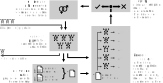
\includegraphics[width=\textwidth]{images/workflow-eacirc}
\caption{Simplified work-flow of the testing process in EACirc.}
\label{fig:workflow-eacirc}
\end{figure}

The initial version of EACirc was created by Petr Švenda at 
the Laboratory of Security and Applied Cryptography, Masaryk University \parencite{labak}.
This initial version provided the main shared functionality: evolutionary capabilities, software circuit emulation
and basic fitness evaluation. Later on, the application was improved by Matej Prišťák and Ondrej Dubovec 
(as their master and bachelor theses, respectively \parencite{thesis-pristak, thesis-dubovec}).

Afterwards, the object model of the entire project was redesigned and a handful of new features was added by myself. 
Most of the code that was taken over was revised and refactored as necessary
to ease the understanding of its function and to standardise naming and programming principles used throughout the project. 
Currently, the framework consist of the following main parts:
\begin{myItemize}
\item \textbf{Evolutionary core}\\
The core evolutionary features are provided by GAlib, a C++ Library of Genetic Algorithm Components developed at MIT \parencite{galib}.
The library, when parametrized by function callbacks (e.\,g.\ function for mutation, sexual crossover, fitness function,~\dots),
handles the main evolutionary actions.
\item \textbf{Circuit emulator}\\
The emulator simulates the behaviour of the circuit loaded from numerical representation. It plays a crucial role in
fitness assessment of the population.
\item \textbf{Project modules}\\
These modules are responsible for generating the data used in circuit fitness assessment. Each module (\textit{project}) corresponds
to one experiment (e.\,g.\ eStream candidate ciphers testing, SHA-3 candidate functions testing, \dots). The module's main
responsibility is to prepare the required number of problem--solution pairs in the form of circuit input stream (problem)
and optimal circuit output (solution). These pair are called a \textit{set of test vectors}.
\item \textbf{Evaluator modules}\\
Evaluator is a function responsible for yielding a numerical value of fitness, when provided with the pairs of
actual and expected circuit outputs. There are multiple approaches to evaluators -- the equality of expected and
actual output can be based on Hamming weight, numerical value, \dots
\item \textbf{Random generators}\\
Since evolutionary algorithms are highly randomized, a source of randomness is needed. To ensure the
computation determinism (all experiments need to be exactly reproducible), a hierarchy of random generators was developed.
To satisfy the varying needs, several generator types are implemented: true quantum random generator (based on pre-generated data),
configurable biased generator and low-entropy MD5-based generator.
\item \textbf{Self-tests}\\
For the ease of development, EACirc provides a handful of self-tests. Running these tests ensures the consistency
of seeding and data manipulation. Tests are implemented using CATCH, a C++ Automated Test Cases in Headers \parencite{catch}.
\item \textbf{XML manipulating library}\\
Most of the files produced and processed by the framework are XML-structured files. All these files are handles via
TinyXML, a simple, small, minimal, C++ XML parser library \parencite{tinyxml}.
\item \textbf{Static checker}\\
The static checker is designed to verify obtained results (evolved circuits) by circumventing both the genetic 
manipulations and circuit emulator. Although  shares some code with the main framework, it is built as an independent application.
\item \textbf{Miscellaneous utilities}\\
EACirc framework comes with an assortment of scripts, used mainly for downloading, checking and processing the results.
\end{myItemize}

\section{Current capabilities of EACirc}
\label{sec:eacirc-capabilities}

EACirc has a variety of other functions improving the core features of evolutionary algorithms and software circuit emulation.
This section provides a short and by no means exhaustive list of them.

\begin{myItemize}
\item \textbf{Bit-reproducibility}\\
Bit-reproducibility is essential for the most research projects, since it enables replication and verification of the results.
EACirc uses genetic programming, which is fundamentally a randomized algorithm. Therefore, a hierarchy of random
generators with strictly defined scope of usage and seeding process was developed. This allowed us to replicate an experiment
by just providing the same input files and a fixed central seed.
\item \textbf{Computation recommencing}\\
After reaching bit-to-bit determinism, we implemented the ability to recommence older computations. 
To allow for this, EACirc was made capable of saving and loading its entire internal state to a set of XML-structured files.
This feature is especially useful for computation-expensive experiments -- when the machine is rebooted, we can continue from last saved state instead of starting all over again.
\item \textbf{Multi-format output}\\
For easy reusing and analysis, the evolved circuits are output in 4 different formats:
\begin{myItemize}
\item binary output (useful for reloading the circuits into EACirc),
\item graph \textsc{dot} output (serves as a visual aid to human analyst),
\item simple text output (application-independent export format) and
\item program output (in the form of a stand-alone C program used for static analysis).
\end{myItemize}
\noindent
The \textsc{dot} graph format can be easily displayed using the Graphviz library \parencite{graphviz} and thus 
facilitates manual analysis done by humans after the computation.\\
This functionality was implemented as early as the first version of EACirc. 
\item \textbf{Static checker for circuits in C}\\
Static checker is used to verify the success of evolved circuits exported as C programs. 
The verification uses pre-generated test vectors
and circumvents most parts of the EACirc framework, mainly the evolution and software circuit emulation.
The independence of this process is of utmost importance, since it provides supporting evidence for the achieved results.
\item \textbf{Modular object model}\\
When redesigning the object model, the principle of modules was utilized, thus enabling integration of multiple projects 
and evaluators according to actual needs. This greatly improved framework's flexibility and extensibility.
Currently, the following three projects (experiments) are implemented:
\begin{myItemize}
\item Project for distinguishing between the output of eStream candidate ciphers and random stream of data was taken from the work of 
Matej Prišťák.
It was slightly revised to operate within the new object model and allow more detailed configuration.
\item Project for distinguishing between the output of SHA-3 candidate functions and random stream of data was inspired by the work of 
Ondrej Dubovec.
Hash functions implementations were taken over, but the test vector generation process was reimplemented from scratch. 
\item A small project for distinguishing among external binary files.
\end{myItemize}
\item \textbf{CUDA support}\\
EACirc supports nVidia CUDA for circuit evaluation during the computation of individual's fitness.
When executed on GPU instead of CPU, the evaluation runtime decreases by the coefficient of about 70.
\end{myItemize}

\noindent
Note, that EACirc is a project beyond the scope of this thesis. Some parts were added and/or redesigned in the process, so
different experiments may have incompatible configuration files and may have produced incomparable results.
For further details, user and development documentation, see EACirc wiki at GitHub \parencite{eacirc-github}.	

\chapter{Experiment settings and output data}
\label{chap:settings}

This chapter summarizes the configuration of EACirc used in the experiments presented in later chapters.
The accounts of random data used are given and EACirc outputs are described. 
In most experiments, our performance is compared to traditional batteries of statistical tests (STS NIST, Dieharder)
therefore settings and output description of these batteries is provided as well.

\section{EACirc settings}
\label{sec:settings-eacirc}

Most of the general settings (evolution and circuit parameters) were taken from Matej Prišťák's thesis \parencite{thesis-pristak}. 
The experiments supporting these parameters values were not reproduced, except for a few -- for details,
see \autoref{chap:distinguish-control}.

The evolution works with a population of 20 individuals, with a sexual crossover probability of 20\,\% and a mutation probability
set to 5\,\%. In each case (if not stated otherwise), we evolve 30\,000 generations with the test vector set
(learning data) changing every 100\textsuperscript{th} generation. Thus, a total of 300 unique test vector sets is used in each run.

The circuit dimensions are limited to 5 layers with a maximum of 8 function nodes per layer. It processes up to 16 input bytes
and produces 2 output bytes. Because of bad experience in previous work, using the \textsc{readx} function is forbidden.
All other implemented functions are allowed.

Each testing set consists of 1\,000 independent vectors, exactly half of which is truly random. 
According to research done by Matej Prišťák, the imbalance in test vectors would make the circuit learn what type is more frequent
in the particular set instead of developing a deterministic distinguisher. 
The order of random and non-random vectors in the set is not fixed.
Hence (\autoref{eq:eacirc-data-use}), all the results output by EACirc are based on a sample of about 2.5\,MB of assessed data.
\begin{equation}
\label{eq:eacirc-data-use}
\Sigma = \frac{30000 \text{ generations}}{100 \; \frac{\text{generations}}{\text{test set}}}
         \cdot \frac{1}{2} \cdot 1000 \; \frac{\text{vector}}{\text{test set}}
         \cdot 16 \; \frac{\text{bytes}}{\text{vector}}
         \approx 2.29 \text{\,MB}
\end{equation}

The expected circuit output is always \texttt{0x00} (zero byte) for a non-random vector and \texttt{0xff} (full byte) 
for a random one.
The used evaluator considers each of the output bytes separately, taking bytes with numerical interpretation lower than
128 as indicating a non-random stream and bytes higher than 127 as indicating a random stream.
Hence, the decision is based only on the first bit of each output byte.
Using the output of the evaluator, the fitness of the circuit is quantified as a quotient of a number of 
correctly predicted vectors and a total number of vectors in a set.

Experiment-specific settings (e.\,g.\ ways of generating non-random stream) are described in the 
appropriate chapters along with the results and their interpretation.

\section{Random data sources}
\label{sec:settings-random}

Eacirc requires a good source of randomness, since the the distinguishing process is based on comparing the assessed data
with a stream of data we declare to be random. All the achieved results therefore rise and fall 
on the quality of this referential stream.

Fortunately, quantum physics provides randomness with inherent unpredictability based on measuring quantum effects of photons. 
We acquired several hundred megabytes of quantum random data from the following on-line services:
\begin{myItemize}
\item \textit{Quantum Random Bit Generation Service}\\
provided by Ruđer Bošković Institute in Zagreb, Croatia \parencite{qrng-service-croatia} and
\item \textit{High Bit Rate Quantum Random Number Generator Service}\\
provided by Humboldt University of Berlin, Germany \parencite{qrng-service-germany}.
\end{myItemize}
The data from both sources have been thoroughly tested and compared, for details and results 
see \autoref{sec:control-germany-croatia}.

\section{EACirc output data}
\label{sec:settings-eacirc-output}

The randomized nature of evolutionary algorithms calls for multiple executions of each experiment due to variation in results.
For the most of the following experiments, we performed 30 independent runs. The final result presented is the average
of these 30 executions.

In each run, the maximum population success rate in the generations just after the change of test vectors are examined.
In our setting, this concerns the 1\textsuperscript{st}, 101\textsuperscript{st}, 201\textsuperscript{st}, \dots{} 
and 29901\textsuperscript{st} generation.
The presented results are of 2 types, depending on how good the found distinguishers are.
\begin{myItemize}
\item If \textit{strong distinguishers} were found, we show the average number of generations needed
to reach them. For our purposes, a population of strong distinguishers has a maximum success rate in generations just
after the change of test vectors over 99\,\% during at least 50 consecutive test vector sets (5\,000 generations).
We call these distinguishers strong, because of their anticipated high success rate on streams they have not been learning on so far.
\item If a population of strong distinguishers was not reached during the evolution, 
we present the average value of maximal success rates in generations just after the change of test vectors,
further averaged across all 30 runs. This average average maximum (\textsc{aam}) is presented in parentheses.
\end{myItemize}

\noindent
In some of the experiments, the results were replicated using the static checker with the evolved circuit.
These sub-experiments always confirmed the qualities of evolved distinguishers and are therefore not presented explicitly
in the result tables.

\section{Settings and output data for statistical test batteries}
\label{sec:settings-statistics}

To compare our results with existing statistical tests, all experiments were replicated using standard batteries of statistical
randomness tests (STS NIST and Dieharder). 
For each setting in EACirc, an external file with 250\,MB of the assessed stream was created.
The same stream was used for both STS NIST and Dieharder tests. For further information on STS NIST and Dieharder, 
see \autoref{chap:stat-rand-testing}.

STS NIST was run on 100 sub-streams, each consisting of 1\,000\,000 bits. This amounts to about 11.92\,MB of assessed data.
All 15 available test were run in all supported configurations. Some runs had problems with tests \textit{Random Excursions} 
and \textit{Random Excursions Variant} (they considered no or less than 100 sub-streams during these test), 
so to ensure statistical accuracy of results, these test are omitted from the results.
For each test, the following results are output:
\begin{myItemize}
\item the number of passed runs (a run is declared failed, if its p-value lies out of the interval determined by the significance
level of $\alpha = 0.01$) and
\item the combined p-value of all 100 runs of the test.
\end{myItemize}
The result of all tests with all supported variants (162 tests in total, 2 tests excluded as mentioned above) 
is summarized in a cumulative score. The score assigns 1 to a test with both number of passed tests and the
combined p-value within the significance interval and assigning 0 otherwise. 
In summary, a fraction of 162/162 denotes a random stream (all tests passed) while a value of 0/162 denotes a highly non-random
stream (no test passed).

From the Dieharder suite, only the test corresponding to the original Diehard collection were used.
The only exception is the \textit{Diehard Sums Test} which was omitted, since the Dieharder community claims it has a couple of
implementation bugs and thus should not be used at all. Each of the chosen tests was rune just once, but was let
to process as much data as it required. Running the whole set processed about 582\,MB altogether with the smallest test
consuming about 3\,MB and the largest one about 127\,MB. Each test was labelled as \textsc{passed}, \textsc{weak} or \textsc{failed}
according to the threshold interval it falls within. The value of $\tau_{weak} = 0.005$ and $\tau_{fail} = 0.000001$ were used.
The result of the whole suite (20 tests in total) is again summarized in a cumulative score assigning 1 to a \textsc{passed} test,
0.5 to a \textsc{weak} test and 0 to a \textsc{failed} test.

\chapter{Control distinguishers}
\label{chap:distinguish-control}

Before performing the experiments themselves, we need to acquire reference results -- what does it mean
streams are indistinguishable from random in out context? Is the referential random data indistinguishable from random?
What is the \textsc{aam} value for the distinguishers?

\section{Looking for non-randomness in quantum random data}
\label{sec:control-random-random}

The first control experiment tries to distinguish quantum random data from other quantum random data.
We use 193\,MB of data obtained from Quantum Random Bit Generator Service (for details, see \autoref{sec:settings-random}).
We presume to fail at this and thus establish the randomness of the assessed data stream.

Using the standard statistical batteries confirmed out expectations -- all 20 tests of Dieharder passed as well as
all 162 tests of STS NIST. Running EACirc yielded the \textsc{aam} value of 0.52 with runs differing in 3\textsuperscript{rd}
or 4\textsuperscript{th} decimal place.

We anticipated that the difference of obtained \textsc{aam} from the naïve value of 0.50 was influenced by population size
and the amount of test vector in a set. This reasoning was based on the following two facts:
\begin{myItemize}
\item \textsc{aam} value is based on fitness of the currently best individual in population (it's a maximum fitness) and thus
larger populations might have a better chance of getting a score above 0.50.
\item With the increasing number of test vectors in a set, the probability of just guessing correctly decreases.
\end{myItemize}

\noindent
The performed experiments (\autoref{tab:random-set-size-change}) confirmed our presumptions: the \textsc{aam} value decreases
with decreasing population size and increasing size of test vector set. We can thus conclude that in our settings the \textsc{aam}
value of 0.52 corresponds to indistinguishable streams.

\begin{table}[h]
\centering
\renewcommand{\arraystretch}{1.2}
\newcolumntype{C}{>{\centering\arraybackslash}X}
\begin{tabularx}{\textwidth}{|c|r||*{6}{C|}} \cline{3-8}
\multicolumn{2}{c||}{} & \multicolumn{6}{c|}{number of test vector in a set} \\ \cline{3-8}
\multicolumn{2}{c||}{} & 200 & 500 & 1000 & 2000 & 5000 & 10\,000 \\ \hline \hline
\multirow{5}*{\rotatedHeader{individuals \\ in population}}
& 5 & -- & -- & (0.509) & - & - & - \\ \cline{2-8}
& 10 & -- & -- & (0.514) & - & - & - \\ \cline{2-8}
& 20 & (0.544) & (0.527) & (0.520) & (0.514) & (0.509) & (0.506) \\ \cline{2-8}
& 50 & - & - & (0.526) & - & - & - \\ \cline{2-8}
& 100 & - & - & (0.530) & - & - & - \\ \hline
\end{tabularx}
\renewcommand{\arraystretch}{1.0}
\caption{Dependence of AAM on population size and test vector set size.}
\label{tab:random-set-size-change}
\end{table}

\section{Distinguishing quantum random data from different sources}
\label{sec:control-germany-croatia}

Secondly, we want to compare quantum random data streams obtained from two different sources (for details, 
see \autoref{sec:settings-random}). We prepared 6 independent files of 5\,MB from each source, and attempted to find
a distinguisher for each pair. The initial reading offset was set to 0 in each of the files so that 
each file produced the same stream every time it was used.

For each pair, the computation was run just once (instead of 30 times). The results are summarized in 
\autoref{tab:control-germany-croatia} -- for each pair the average of the maximum population fitness in the generations
just after the test vector change is displayed (this would correspond to the \textsc{aam} value, if 30 runs
were performed for each pair).

The results oscillate closely around 0.52 indicating indistinguishable streams (see \autoref{sec:control-random-random}).
We can thus conclude that, for our purposes, both sources are equally random and equally reliable. 
Since no of the tested files expressed any statistically significant deviation from the others, we can use these files
interchangeably.

\begin{table}[h]
\centering
\renewcommand{\arraystretch}{1.2}
\newcolumntype{C}{>{\centering\arraybackslash}X}
\begin{tabularx}{\textwidth}{|c|r||*{6}{C|}} \cline{3-8}
\multicolumn{2}{c||}{} & \multicolumn{6}{c|}{QRBG service (Ruđer Bošković Institute, Croatia)} \\ \cline{3-8}
\multicolumn{2}{c||}{} & stream 1 & stream 2 & stream 3 & stream 4 & stream 5 & stream 6 \\ \hline \hline
\multirow{6}*{\rotatedHeader{QRNG service \\(HU, Germany)}}
& stream 1 & (0.521) & (0.520) & (0.520) & (0.519) & (0.519) & (0.519) \\ \cline{2-8}
& stream 2 & (0.518) & (0.519) & (0.520) & (0.520) & (0.520) & (0.519) \\ \cline{2-8}
& stream 3 & (0.519) & (0.522) & (0.519) & (0.520) & (0.519) & (0.519) \\ \cline{2-8}
& stream 4 & (0.520) & (0.520) & (0.519) & (0.518) & (0.519) & (0.519) \\ \cline{2-8}
& stream 5 & (0.519) & (0.520) & (0.519) & (0.518) & (0.520) & (0.520) \\ \cline{2-8}
& stream 6 & (0.520) & (0.519) & (0.520) & (0.520) & (0.519) & (0.519) \\ \hline
\end{tabularx}
\renewcommand{\arraystretch}{1.0}
\caption{Distinguishing binary quantum random streams from independent sources.}
\label{tab:control-germany-croatia}
\end{table}

\section{Uncompressed audio streams}
\label{sec:distinguishing-audio}

The third and last of the control experiments compares the set of audio files. We considered a set of 12 files -- 3 quantum random
data files, 3 uncompressed audio files with white, pink and Brownian noise, the same noise files with intermediate mp3 compression
and 3 samples of uncompressed black-metal music.

The quantum random data files had about 5\,MB and were turned into a listenable file by adding a \textsc{wav} header 
instructing to interpret the data as 2-channel, 16\,bit/sample, 44.1\,kHz PCM-encoded audio.
The 30 seconds (about 5.3\,MB) samples of white, pink and Brownian noise in the same audio format were generated using SoX
\parencite{sox}. The third subset was created from the above-mentioned generated noises by mp3 compression (bitrate of 
128\,kbps) and decompression back to the PCM-encoded audio. Note, that after compression the files
took about 480\,kB each (compared to 5.3\,MB of the uncompressed version).
The last three were 30 seconds samples of transcendental khaoblack metal by Abbey ov Thelema \parencite{abbey-ov-thelema}
all taken from the band's promo called \textit{MMXII: Here \& Now - At the Threshold ov End Times}.

We again attempted to develop a distinguisher for each pair of these files, again setting initial reading offset to 0
and performing just one execution per file combination. Our hypotheses included the following:
\begin{myItemize}
\item the quantum random files will be indistinguishable from each other (assumption based on results from 
\autoref{sec:control-germany-croatia}),
\item the noise will be very similar to quantum random data (especially the white noise), but it may be able to be told apart,
\item the different noise types will be similar to each other,
\item the compressed and decompressed noise will be easily distinguishable from both the uncompressed noise and quantum random data
files (even though they cannot be easily differentiated by human ear),
\item the provided samples of metal music will be equally easily told apart from the other files, both uncompressed and re-compressed.
\end{myItemize}

\noindent
The results are presented in the usual way in \autoref{tab:control-audio} (the part below the diagonal is mirrored to
facilitate analysis). From the analysis the the values, we accept most of the hypotheses:
\begin{myItemize}
\item quantum random stream are undistinguishable (average maximum success rate of 0.52, see \autoref{sec:control-random-random}
for details),
\item generated white noise is completely undistinguishable from random data files,
\item pink and Brownian noise are easily told apart from each other or the quantum random files (success rate generally over 80\,\%),
\item mp3 compression has small, but detectable effect on the sound (although nearly undetectable by unskilled human ear, 
it successfully shifts the distinguisher success rate to about 0.58 when comparing with an uncompressed noise of the same kind),
\item used metal samples can be reliably distinguished from white noise (general success over 80\,\%), 
less so from pink and Brownian noise (success rate only around 65\,\%),
\item used metal samples are nearly indistinguishable from each other on the binary level 
(although the differences are easily detectable by human ear).
\end{myItemize}

\begin{landscape}
\begin{table}[p]
\centering
\newsavebox{\temp}
\newcolumntype{C}{>{\centering \begin{lrbox}{\temp} \arraybackslash}X<{\end{lrbox} \m{\unhbox\temp} \arraybackslash}}
\begin{tabularx}{22cm}{|c|>{\raggedright\arraybackslash}p{2.5cm}*{4}{||C|C|C}|} \cline{3-14}

\multicolumn{2}{l||}{} & \multicolumn{3}{c||}{random streams} & \multicolumn{3}{c||}{noise (true)} &
\multicolumn{3}{c||}{noise (via mp3)} & \multicolumn{3}{c|}{metal music} \\ \cline{3-14}

\multicolumn{2}{l||}{} &  
\multicolumn{1}{c|}{\rotatedHeader{random\\stream 1}} & 
\multicolumn{1}{c|}{\rotatedHeader{random\\stream 2}} & 
\multicolumn{1}{c||}{\rotatedHeader{random\\stream 3}} & 
\multicolumn{1}{c|}{\rotatedHeader{white noise}} & 
\multicolumn{1}{c|}{\rotatedHeader{pink noise}} & 
\multicolumn{1}{c||}{\rotatedHeader{Brown noise}} & 
\multicolumn{1}{c|}{\rotatedHeader{white noise\\(via mp3)}} & 
\multicolumn{1}{c|}{\rotatedHeader{pink noise\\(via mp3)}} & 
\multicolumn{1}{c||}{\rotatedHeader{brown noise\\(via mp3)}} & 
\multicolumn{1}{c|}{\rotatedHeader{metal music\\(sample 1)}} & 
\multicolumn{1}{c|}{\rotatedHeader{metal music\\(sample 2)}} & 
\multicolumn{1}{c|}{\rotatedHeader{metal music\\(sample 3)}} \\ \cline{3-14} \hline \hline

\multirow{3}{*}[-20pt]{\rotatedHeader{random}} &
random stream 1 & 
n/a & (0.52) & (0.52) & (0.52) & (0.80) & (0.84) & (0.59) & (0.93) & (0.89) & (0.84) & (0.87) & (0.83) \\ \cline{2-14}
& random stream 2 &
(0.52) & n/a & (0.52) & (0.52) & (0.83) & (0.83) & (0.57) & (0.82) & (0.84) & (0.90) & (0.85) & (0.82) \\ \cline{2-14}
& random stream 3 & 
(0.52) & (0.52) & n/a & (0.52) & (0.94) & (0.91) & (0.58) & (0.83) & (0.83) & (0.89) & (0.83) & (0.85) \\ \hline \hline
\multirow{3}{*}[-10pt]{\rotatedHeader{noise (true)}} & 
white noise (true) &
(0.52) & (0.52) & (0.52) & n/a & (0.83) & (0.81) & (0.59) & (0.87) & (0.89) & (0.86) & (0.93) & (0.81) \\ \cline{2-14}
& pink noise (true) &
(0.80) & (0.83) & (0.94) & (0.83) & n/a & (0.76) & (0.86) & (0.52) & (0.76) & (0.65) & (0.65) & (0.66) \\ \cline{2-14}
& Brown noise (true) &
(0.84) & (0.83) & (0.91) & (0.81) & (0.76) & n/a & (0.86) & (0.76) & (0.56) & (0.71) & (0.69) & (0.68) \\ \hline \hline
\multirow{3}{*}[-10pt]{\rotatedHeader{noise (mp3)}} & 
white noise (via mp3) &
(0.59) & (0.57) & (0.58) & (0.59) & (0.86) & (0.86) & n/a & (0.91) & (0.83) & (0.84) & (0.80) & (0.78) \\ \cline{2-14}
& pink noise (via mp3) &
(0.93) & (0.82) & (0.83) & (0.87) & (0.52) & (0.76) & (0.91) & n/a & (0.78) & (0.63) & (0.68) & (0.70) \\ \cline{2-14}
& Brown noise (via mp3) &
(0.89) & (0.84) & (0.83) & (0.89) & (0.76) & (0.56) & (0.83) & (0.78) & n/a & (0.71) & (0.69) & (0.67) \\ \hline \hline
\multirow{3}{*}[-5pt]{\rotatedHeader{metal music}} & 
metal music (sample 1) &
(0.84) & (0.90) & (0.89) & (0.86) & (0.65) & (0.71) & (0.84) & (0.63) & (0.71) & n/a & (0.54) & (0.56) \\ \cline{2-14}
& metal music (sample 2) &
(0.87) & (0.85) & (0.83) & (0.93) & (0.65) & (0.69) & (0.80) & (0.68) & (0.69) & (0.54) & n/a & (0.53) \\ \cline{2-14}
& metal music (sample 3) &
(0.83) & (0.82) & (0.85) & (0.81) & (0.66) & (0.68) & (0.78) & (0.70) & (0.67) & (0.56) & (0.53) & n/a \\ \cline{1-14}
\end{tabularx}
\caption{Distinguishing random streams and uncompressed audio (noise, compressed noise, metal music).}
\label{tab:control-audio}
\end{table}
\end{landscape}

\chapter{Distinguishing cipher outputs from random stream}
\label{chap:distinguish-cipher}

Inspired by the research done by Matej Prišťák \parencite{thesis-pristak}, we analysed randomness of stream cipher outputs.
The analysis used either EACirc, Dieharder or STS NIST with settings described earlier (\autoref{chap:settings}).
We only considered stream ciphers from the recent eStream competition \parencite{estream-competition},
since we could use the unified cipher interface (API) prescribed in the competition.

\section{Generating binary stream from stream ciphers}
\label{sec:estream-settings}

From 34 candidates in the eStream competition, 23 were potentially usable for testing (due to renamed or updated versions, 
problems with compilation,~\dots). Out of these, we limited ourselves to only 7 (Decim, Grain, FUBUKI, Hermes, LEX, Salsa20 and TSC),
since these had internal structure that allowed for a simple reduction of complexity by reducing a number of internal rounds.
For all used ciphers, the implementation from the last successful phase of the competition was taken. 
The ciphers were tested unlimited and then for all lower number of rounds until reaching distinguishability from a random stream.

As opposed to our previous research, we considered three modes with respect to the frequency of cipher initialization and key change:
\begin{myItemize}
\item The cipher initialization is performed just once (at the beginning of the computation) and the key is fixed for
all the generated test vectors and sets. Even when the sets change, new test vectors are generated using the same key.
\item Every test set is generated using different key. All test vectors in a particular set are generated with the same key.
The cipher is reinitialized when the key is changed, i.\,e.\ at set change.
\item Every single test vector is generated using a different key and a freshly initialized cipher.
\end{myItemize}
For every setting, each mode was considered separately. Keys were generated randomly and initialization vectors and plaintexts
were fixed to binary zeroes.

\section{Results interpretation}
\label{sec:estream-results}

Before coming to the results, two things must be noted:
\begin{myItemize}
\item The internal structure of LEX responds specifically to the limitation of number of rounds.
LEX prepares 4 output bytes during every round (other bytes default to binary zero). 
Limitation of internal rounds therefore only limits the number
of output bytes, not their strength/randomness.
\item During the first 8 rounds, TSC only fills internal memory structures and thus produces no output. The output of these rounds
is therefore a default stream of binary zeroes. Such stream also causes 4 of the Dieharder tests to get stuck --
the score from the remaining 16 tests is presented with an asterisk (*).
\end{myItemize}

\noindent
The results of the described distinguisher experiments can be seen in \autoref{tab:estream-grain} to
\autoref{tab:estream-tsc}. The value of $n$ indicates average number of generations needed to reach a population of
strong distinguishers while the number in parentheses expresses the \textsc{aam} value in case such a generation has not been
found. For detailed description of the data meanings see \autoref{sec:settings-eacirc-output}. We also remind the reader
that the value of 0.52 indicates the stream is indistinguishable from random (for reasoning, see \autoref{sec:control-random-random}).

In summary, the results indicate that in this case, EACirc performs more or less the same as standard statistical batteries.
Although it did not always find a population of strong distinguishers, it found a population with significantly better
success rate than random guessing in most of the cases (Decim being the most prominent exception).
Dieharder sometimes performed better than STS NIST, but it has to be taken into consideration that it is newer
and made decision based on a much larger sample. In general, both statistical batteries processed longer stream than EACirc
(for detailed numbers see \autoref{chap:settings}). Regarding the matters of speed, EACirc had a comparably longer learning phase,
but usually provided a distinguisher working working in far less time than statistical batteries.
\medskip

\begin{table}[hb]
\centering
\resultsTableEstream{
1 & 0.0 & 0 & $n=2681$ & 0.0 & 0 & (0.85) & 0.0 & 5 & $n=1431$ \\ \hline
2 & 0.5 & 0 & (0.54) & 1.0 & 0 & (0.54) & 15.5 & 146 & (0.52) \\ \hline
3 & 1.0 & 0 & (0.53) & 1.0 & 0 & (0.53) & 15.0 & 160 & (0.52) \\ \hline
4 & 3.5 & 79 & (0.52) & 3.0 & 78 & (0.52) & 20.0 & 160 & (0.52) \\ \hline
5 & 4.5 & 79 & (0.52) & 3.5 & 91 & (0.52) & 17.5 & 161 & (0.52) \\ \hline
6 & 19.0 & 158 & (0.52) & 19.0 & 159 & (0.52) & 18.0 & 162 & (0.52) \\ \hline
7 & 18.5 & 162 & (0.52) & 19.0 & 161 & (0.52) & 20.0 & 161 & (0.52) \\ \hline \hline
8 & 20.0 & 162 & (0.52) & 20.0 & 159 & (0.52) & 19.0 & 161 & (0.52) \\ \hline
}
\caption{Random distinguishers for Decim ciphertext.}
\label{tab:estream-decim}
\end{table}

\begin{table}[htb]
\centering
\resultsTableEstream{
1 & 20.0 & 162 & (0.52) & 20.0 & 161 & (0.52) & 18.0 & 162 & (0.52) \\ \hline \hline
4 & 20.0 & 162 & (0.52) & 20.0 & 162 & (0.52) & 20.0 & 162 & (0.52) \\ \hline
}
\caption{Random distinguishers for FUBUKI ciphertext.}
\label{tab:estream-fubuki}
\end{table}

\begin{table}[htb]
\centering
\resultsTableEstream{
1 & 0.0 & 0 & $n=221$ & 0.0 & 0 & (0.67) & 18.5 & 162 & (0.52) \\ \hline
2 & 0.0 & 0 & $n=471$ & 0.5 & 0 & (0.66) & 20.0 & 162 & (0.52) \\ \hline
3 & 19.5 & 160 & (0.52) & 20.0 & 162 & (0.52) & 20.0 & 162 & (0.52) \\ \hline \hline
13 & 20.0 & 162 & (0.52) & 20.0 & 161 & (0.52) & 19.5 & 162 & (0.52) \\ \hline
}
\caption{Random distinguishers for Grain ciphertext.}
\label{tab:estream-grain}
\end{table}

\begin{table}[htb]
\centering
\resultsTableEstream{
1 & 20.0 & 162 & (0.52) & 20.0 & 162 & (0.52) & 20.0 & 162 & (0.52) \\ \hline \hline
10 & 20.0 & 160 & (0.52) & 20.0 & 162 & (0.52) & 20.0 & 162 & (0.52) \\ \hline
}
\caption{Random distinguishers for Hermes ciphertext.}
\label{tab:estream-hermes}
\end{table}

\begin{table}[htb]
\centering
\resultsTableEstream{
1 & 0.0 & 0 & $n=148$ & 0.0 & 0 & $n=7274$ & 3.0 & 1${}^{*}$ & $n=154$ \\ \hline
2 & 4.0 & 1 & $n=221$ & 4.0 & 1 & $n=304$ & 3.5 & 1 & $n=254$ \\ \hline
3 & 0.5 & 1 & $n=378$ & 3.5 & 1 & $n=491$ & 4.0 & 1 & $n=361$ \\ \hline
4 & 20.0 & 162 & (0.52) & 19.5 & 162 & (0.52) & 20.0 & 161 & (0.52) \\ \hline \hline
10 & 19.5 & 162 & (0.52) & 19.5 & 160 & (0.52) & 20.0 & 160 & (0.52) \\ \hline
}
\caption{Random distinguishers for LEX ciphertext.}
\label{tab:estream-lex}
\end{table}

\begin{table}[htb]
\centering
\resultsTableEstream{
1 & 5.5 & 1 & (0.87) & 8.5 & 1 & (0.67) & 17.5 & 161 & (0.52) \\ \hline
2 & 5.5 & 1 & (0.87) & 7.0 & 1 & (0.67) & 19.5 & 162 & (0.52) \\ \hline
3 & 20.0 & 162 & (0.52) & 20.0 & 162 & (0.52) & 19.5 & 161 & (0.52) \\ \hline \hline
12 & 20.0 & 162 & (0.52) & 19.5 & 161 & (0.52) & 19.0 & 161 & (0.52) \\ \hline
}
\caption{Random distinguishers for Salsa20 ciphertext.}
\label{tab:estream-salsa}
\end{table}

\begin{table}[htb]
\centering
\resultsTableEstream{
1--8 & 0.0${}^{*}$ & 0 & $n=104$ & 0.0${}^{*}$ & 0 & $n=101$ & 0.0${}^{*}$ & 0 & $n=104$ \\ \hline
9 & 1.0 & 1 & $n=234$ & 1.5 & 1 & $n=491$ & 2.0 & 1 & $n=121$ \\ \hline
10 & 2.0 & 13 & $n=188$ & 3.0 & 13 & $n=218$ & 3.0 & 12 & $n=158$ \\ \hline
11 & 10.0 & 157 & (0.52) & 11.5 & 157 & (0.52) & 14.0 & 159 & (0.52) \\ \hline
12 & 16.0 & 162 & (0.52) & 17.0 & 161 & (0.52) & 17.5 & 162 & (0.52) \\ \hline
13 & 20.0 & 162 & (0.52) & 20.0 & 162 & (0.52) & 19.0 & 162 & (0.52) \\ \hline \hline
32 & 20.0 & 161 & (0.52) & 20.0 & 162 & (0.52) & 20.0 & 161 & (0.52) \\ \hline
}
\caption{Random distinguishers for TSC-4 ciphertext.}
\label{tab:estream-tsc}
\end{table}

\chapter{Analysis of Salsa20 output stream}
\label{chap:analysis-salsa}
\begin{myItemize}
\item learns current vectors quicker than other ciphers
\item the case of six, see \autoref{fig:salsa20-case1}
\end{myItemize}

\begin{figure}[b!]
\centering
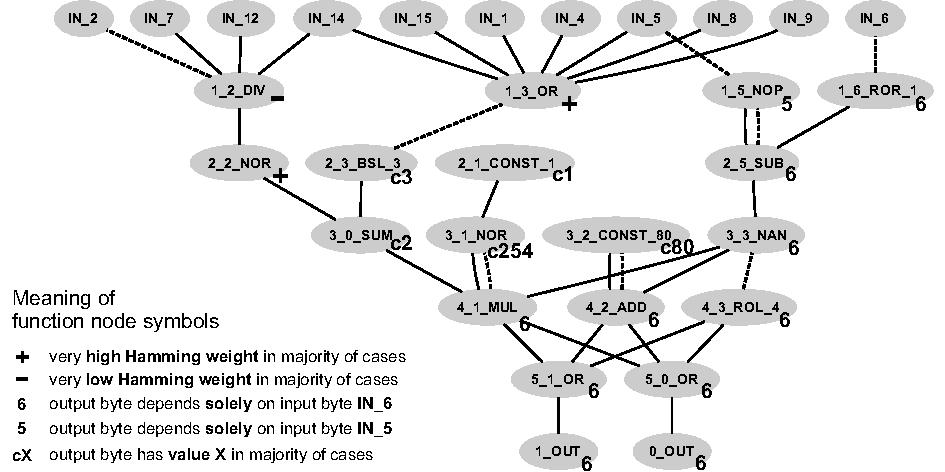
\includegraphics[width=\textwidth]{images/case1-final}
\caption{Analysis of a distinguisher evolved for Salsa20 limited to 2 rounds (pruned version of the circuit is displayed).}
\label{fig:salsa20-case1}
\end{figure}

\chapter{Distinguishing hash outputs from random stream}
\label{chap:distinguish-hash}

Similar experiments as done in \autoref{chap:distinguish-cipher} were performed on candidate hash functions from SHA-3 competition
\parencite{sha3-competition}
(inspired by research done by Ondrej Dubovec \parencite{thesis-dubovec}).
As in eStream ciphers, we utilized the unified hash function interface (API) prescribed in the competition.
We analysed the randomness of streams produces as a concatenation of hash digests.
The usual settings for EACirc, Dieharder and STS NIST were used (see \autoref{chap:settings} for details).

\section{Generating stream from hash function outputs}
\label{sec:hash-settings}

From 64 hash functions that entered the competition, 51 were selected to the first round. 
Out of these, 42 were potentially usable for testing (due to source code size, speed and compilation problems).
The implementations (taken from the last successful phase of the competition) and
modifications limiting the number of rounds in these functions were taken over from previous work \parencite{thesis-dubovec}
and revised. In the end, 18 most promising candidates were chosen: ARIRANG, Aurora, Blake, Cheetah, CubeHash, DCH, 
Dynamic SHA, Dynamic SHA2, ECHO, Grøstl, Hamsi, JH, Lesamnta, Luffa, MD6, SIMD, Tangle, and Twister.
These were the candidates which could be successfully limited in complexity and while their full version produced a random-looking
output, their most limited version did not. All these hash function were subsequently tested unlimited and
then for all lower number of rounds until reaching distinguishability from a random stream.

As opposed to the work we were inspired by, we generated continuous output stream by hashing a simple 4-byte counter starting
from a randomly generated value. We obtained a 256-bit digest, which we cut in half to produce 2 independent test vector inputs
of 16 bytes each. In case of generating a continuous stream (for the purposes of Dieharder and STS NIST), we concatenated 
the digests.

\section{Determining optimal set change frequency}
\label{sec:hash-set-change-freqency}

In the previous work \parencite{thesis-dubovec}, Ondrej Dubovec claims that optimal test set change frequency is once
per 10 generations. However, not enough evidence supporting this hypothesis is provided. Since in other experiments in this thesis
we changed test vector set once in 100 generations (a setting taken over from Matej Prišťák's work \parencite{thesis-pristak}), 
we decided to re-test the optimality of this setting.

We performed reference computation on Dynamic SHA limited to 5 rounds. The \textsc{aam} values for the usual 30\,000 generations
along with the estimate runtime are displayed in the first two rows of \autoref{tab:hash-set-change-freqency}.
From these results it seems that decreasing the test set use period increases the success rate, which we considered slightly
counter-intuitive (since the circuits work with the same vectors only for a very limited time).

It must noted, however, that circuits in these experiments had extremely different amounts of data -- only 30 sets of test vectors
in case of changing the set once in 1\,000 generations compared to astounding 6\,000 different test sets when changing every 
5\textsuperscript{th} generation. To even out these differences, we re-run the experiments while using exactly 300 unique test sets
in each case. The results can be seen in the bottom two lines of the same table. In this case we see a completely reversed
behaviour.

All in all, we decided to keep the setting of changing the test set every 100\textsuperscript{th} generation.
Doing so is a acceptable trade-off between circuit success rate and required run time. 
Furthermore, we retain settings similar to the previous experiments, which facilitates the comparison of the results.
\bigskip

\begin{table}[htb]
\centering
\renewcommand{\arraystretch}{1.2}
\newcolumntype{C}{>{\centering\arraybackslash}X}
\begin{tabularx}{\textwidth}{|>{\raggedright\arraybackslash}p{2cm}||*{8}{C|}} \cline{2-9}
\multicolumn{1}{l||}{} & \multicolumn{8}{c|}{change frequency for test vector set} \\ \cline{2-9}
\multicolumn{1}{l||}{} & 5 & 10 & 20 & 50 & 100 & 200 & 500 & 1000 \\ \hline \hline
30\,000 gen. & (0.614) & (0.614) & (0.607) & (0.602) & (0.599) & (0.598) & (0.591) & (0.582) \\ \hline
run-time & 70 m. & 52 m. & 42 m. & 37 m. & 32 m. & 28 m. & 23 m. & 20 m. \\ \hline \hline
300 sets & (0.567) & (0.583) & (0.585) & (0.589) & (0.599) & (0.608) & (0.617) & (0.618) \\ \hline
run-time & 4 m. & 6 m. & 9 m. & 19 m. & 32 m. & 57 m. & 115 m. & 220 m. \\ \hline
\end{tabularx}
\renewcommand{\arraystretch}{1.0}
\caption{Determining optimal change frequency for test vector set.}
\label{tab:hash-set-change-freqency}
\end{table}

\section{Results interpretation}
\label{sec:hash-results}

The results of the above-introduced experiments are summarized in \autoref{tab:sha3-arirang} to \autoref{tab:sha3-twister} 
in the usual way. 
The value of $n$ indicates average number of generations needed to reach a population of
strong distinguishers while the number in parentheses expresses the \textsc{aam} value in case such a generation has not been
found. For detailed description of the data meanings see \autoref{sec:settings-eacirc-output}. 
A number in brackets following the average generation indicates that only this many
out of total 30 runs reached a stable population of strong distinguishers. We also remind the reader
that the value of 0.52 indicates the stream is indistinguishable from random (for reasoning, see \autoref{sec:control-random-random}).

Notice the asterisk in Dieharder results in \autoref{tab:sha3-dch} and \autoref{tab:sha3-md6}.
In these cases, the hash functions produced no output at all (output stream defaulted to binary zero).
This caused 4 Dieharder tests to get stuck, effectively reducing the number of tests to 16 
(situation similar to \autoref{tab:estream-tsc}).

In summary, the results indicate that in this case, EACirc performs slightly worse than standard statistical batteries.
Although in most of the cases it either found a population of strong distinguishers or a statistically significant variation
from a neutral success rate of 0.52, it can be seen that it often failed in the last round successfully distinguished
by statistical batteries. Once again, when interpreting these results, we must be aware of the imbalance of test data
available to statistical batteries and EACirc (for detailed numbers see \autoref{chap:settings}).

Another observation worth noting is the consistency of the results within the 30 runs of the same experiment.
Previously (mainly \autoref{chap:distinguish-cipher}), all the results within an experiment were consistent 
(all 30 runs reached more or less the same results).
The computations presented in this chapter display the variations characteristic to evolutionary algorithms -- 
only some of the runs are successful (the randomized evolution in the other just did not succeed).
It may be interesting to consider a larger amount of runs in border cases, where statistical batteries were successful
but EACirc was not.
\vfill

\begin{table}[h]
\twoColumns{
\resultsTableSha{
0 & 0.0 & 0 & $n=694$ \\ \hline
1 & 0.0 & 0 & $n=707$ \\ \hline
2 & 0.0 & 0 & $n=467$ \\ \hline
3 & 0.0 & 0 & $n=1071$ \\ \hline \hline
4 & 20.0 & 161 & (0.52) \\ \hline
}
\caption{Random distinguishers for ARIRANG output.}
\label{tab:sha3-arirang}
\bigskip
\resultsTableSha{
0 & 0.0 & 1 & $n=5614$ \\ \hline
1 & 0.0 & 1 & $n=4101$ [1] \\ \hline
2 & 0.5 & 132 & $n=13201$ [1] \\ \hline
3 & 0.5 & 132 & (0.52) \\ \hline
4 & 20.0 & 160 & (0.52) \\ \hline \hline
17 & 19.5 & 161 & (0.52) \\ \hline
}
\caption{Random distinguishers for Aurora output.}
\label{tab:sha3-aurora}
}{
\resultsTableSha{
0 & 0.0 & 0 & $n=474$ \\ \hline
1 & 0.0 & 0 & (0.52) \\ \hline
2 & 20.0 & 162 & (0.52) \\ \hline \hline
14 & 20.0 & 159 & (0.52) \\ \hline
}
\caption{Random distinguishers for Blake output.}
\label{tab:sha3-blake}
\bigskip
\resultsTableSha{
0 & 0.0 & 1 & $n=181$ \\ \hline
1 & 0.0 & 1 & $n=574$ \\ \hline
2 & 0.0 & 0 & $n=708$ \\ \hline
3 & 0.0 & 0 & $n=14659$ [12] \\ \hline
4 & 0.0 & 1 & $n=16870$ [10] \\ \hline
5 & 0.0 & 1 & (0.52) \\ \hline
6 & 20.0 & 161 & (0.52) \\ \hline \hline
16 & 20.0 & 162 & (0.52) \\ \hline
}
\caption{Random distinguishers for Cheetah output.}
\label{tab:sha3-cheetah}
}
\end{table}

\begin{table}[htb]
\twoColumns{
\resultsTableSha{
0 & 0.0 & 0 & $n=104$ \\ \hline
1 & 0.0 & 0 & (0.52) \\ \hline
2 & 20.0 & 161 & (0.52) \\ \hline \hline
8 & 20.0 & 162 & (0.52) \\ \hline
}
\caption{Random distinguishers for CubeHash output.}
\label{tab:sha3-cubehash}
\bigskip
\resultsTableSha{
0 & 0.0${}^{*}$ & 0 & $n=104$ \\ \hline
1 & 0.0${}^{*}$ & 0 & $n=17260$ [5] \\ \hline
2 & 19.5 & 162 & (0.52) \\ \hline
4 & 20.0 & 162 & (0.52) \\ \hline
}
\caption{Random distinguishers for DCH output.}
\label{tab:sha3-dch}
\bigskip
\resultsTableSha{
0 & 0.0 & 0 & $n=484$ \\ \hline
1 & 0.0 & 0 & $n=2337$ \\ \hline
2 & 0.0 & 1 & $n=1773$ \\ \hline
3 & 0.0 & 1 & $n=12731$ [10] \\ \hline
4 & 0.0 & 18 & (0.74) \\ \hline
5 & 0.5 & 18 & (0.61) \\ \hline
6 & 3.0 & 16 & (0.59) \\ \hline
7 & 3.0 & 17 & (0.59) \\ \hline
8 & 20.0 & 162 & (0.52) \\ \hline \hline
16 & 20.0 & 160 & (0.52) \\ \hline
}
\caption{Random distinguishers for Dynamic SHA output.}
\label{tab:sha3-dsha}
}{
\resultsTableSha{
1 & 1.0 & 1 & $n=15886$ [13] \\ \hline
2 & 1.0 & 1 & (0.74) \\ \hline
3 & 0.0 & 1 & (0.75) \\ \hline
4 & 0.0 & 1 & (0.57) \\ \hline
5 & 3.5 & 1 & (0.60) \\ \hline
6 & 3.5 & 1 & (0.60) \\ \hline
7 & 4.0 & 2 & (0.61) \\ \hline 
8 & 4.0 & 2 & (0.60) \\ \hline
9 & 3.5 & 5 & (0.61) \\ \hline
10 & 3.5 & 5 & (0.61) \\ \hline
11 & 11.5 & 46 & (0.52) \\ \hline
12 & 11.5 & 46 & (0.52) \\ \hline
13 & 20.0 & 161 & (0.52) \\ \hline \hline
17 & 20.0 & 161 & (0.52) \\ \hline
}
\caption{Random distinguishers for Dynamic SHA2 output.}
\label{tab:sha3-dsha2}
\bigskip
\resultsTableSha{
1 & 9.0 & 24 & $n=10501$ [3] \\ \hline
2 & 9.0 & 24 & (0.52) \\ \hline
3 & 20.0 & 161 & (0.52) \\ \hline \hline
8 & 20.0 & 161 & (0.52) \\ \hline
}
\caption{Random distinguishers for ECHO output.}
\label{tab:sha3-echo}
}
\end{table}

\begin{table}[htb]
\twoColumns{
\resultsTableSha{
0 & 0.0 & 0 & $n=6285$ [25] \\ \hline
1 & 0.0 & 0 & (0.58) \\ \hline
2 & 12.5 & 52 & (0.58) \\ \hline
3 & 12.5 & 52 & (0.52) \\ \hline
4 & 20.0 & 162 & (0.52) \\ \hline \hline
10 & 20.0 & 162 & (0.52) \\ \hline
}
\caption{Random distinguishers for Grøstl output.}
\label{tab:sha3-grostl}
\bigskip
\resultsTableSha{
0 & 2.5 & 1 & $n=10376$ [24] \\ \hline
1 & 2.5 & 1 & (0.52) \\ \hline
2 & 19.5 & 161 & (0.52) \\ \hline \hline
3 & 20.0 & 162 & (0.52) \\ \hline
}
\caption{Random distinguishers for Hamsi output.}
\label{tab:sha3-hamsi}
\bigskip
\resultsTableSha{
0 & 0.0 & 0 & $n=581$ \\ \hline
1 & 0.0 & 0 & $n=4397$ \\ \hline
2 & 0.0 & 1 & $n=5984$ \\ \hline
3 & 0.0 & 1 & $n=3674$ \\ \hline
4 & 0.0 & 1 & $n=1748$ \\ \hline
5 & 0.0 & 3 & $n=784$ \\ \hline
6 & 0.0 & 3 & $n=5040$ [28] \\ \hline
7 & 20.0 & 161 & (0.52) \\ \hline \hline
42 & 20.0 & 162 & (0.52) \\ \hline
}
\caption{Random distinguishers for JH output.}
\label{tab:sha3-jh}
}{
\resultsTableSha{
0 & 0.0 & 0 & $n=791$ \\ \hline
1 & 0.0 & 0 & $n=568$ \\ \hline
2 & 0.0 & 0 & $n=504$ \\ \hline
3 & 0.0 & 0 & (0.52) \\ \hline
4 & 20.0 & 162 & (0.52) \\ \hline \hline
32 & 20.0 & 162 & (0.52) \\ \hline
}
\caption{Random distinguishers for Lesamnta  output.}
\label{tab:sha3-lesamnta}
\bigskip
\resultsTableSha{
0 & 0.0 & 0 & $n=604$ \\ \hline
1 & 0.0 & 0 & $n=1073$ [29] \\ \hline
2 & 0.0 & 1 & $n=2074$ \\ \hline
3 & 0.0 & 1 & $n=3735$ [29] \\ \hline
4 & 0.0 & 4 & (0.75) \\ \hline
5 & 0.0 & 3 & (0.75) \\ \hline
6 & 0.0 & 10 & (0.74) \\ \hline
7 & 6.0 & 11 & (0.74) \\ \hline \hline
8 & 20.0 & 161 & (0.52) \\ \hline
}
\caption{Random distinguishers for Luffa output.}
\label{tab:sha3-luffa}
}
\end{table}

\begin{table}[htb]
\twoColumns{
\resultsTableSha{
0 & 0.0${}^{*}$ & 0 & $n=101$ \\ \hline
1 & 0.0${}^{*}$ & 0 & $n=1281$ \\ \hline
2 & 0.0 & 0 & $n=1084$ \\ \hline
3 & 0.0 & 0 & $n=631$ \\ \hline
4 & 0.0 & 0 & $n=781$ \\ \hline
5 & 0.0 & 0 & $n=13020$ [21] \\ \hline
6 & 0.0 & 1 & (0.88) \\ \hline
7 & 0.0 & 1 & (0.65) \\ \hline
8 & 17.5 & 18 & (0.53) \\ \hline
9 & 17.5 & 18 & (0.52) \\ \hline
10 & 20.0 & 160 & (0.52) \\ \hline \hline
104 & 20.0 & 162 & (0.52) \\ \hline
}
\caption{Random distinguishers for MD6 output.}
\label{tab:sha3-md6}
\bigskip
\resultsTableSha{
0 & 0.0 & 0 & $n=474$ \\ \hline
1 & 0.0 & 0 & $n=718$ \\ \hline
2 & 0.0 & 0 & $n=524$ \\ \hline
3 & 0.0 & 0 & $n=1247$ \\ \hline
4 & 0.0 & 0 & $n=1334$ \\ \hline
5 & 0.0 & 0 & $n=411$ \\ \hline
6 & 0.0 & 0 & $n=524$ \\ \hline
7 & 0.0 & 0 & (0.52) \\ \hline
8 & 20.0 & 161 & (0.52) \\ \hline \hline
9 & 20.0 & 162 & (0.52) \\ \hline
}
\caption{Random distinguishers for Twister output.}
\label{tab:sha3-twister}
}{
\resultsTableSha{
0 & 0.0 & 1 & $n=4697$ [28] \\ \hline
1 & 0.0 & 1 & (0.52) \\ \hline
2 & 19.5 & 162 & (0.52) \\ \hline \hline
4 & 19.5 & 161 & (0.52) \\ \hline
}
\caption{Random distinguishers for SIMD output.}
\label{tab:sha3-simd}
\bigskip
\resultsTableSha{
0 & 0.0 & 0 & $n=714$ \\ \hline
1 & 0.0 & 0 & $n=6868$ \\ \hline
2 & 0.0 & 1 & $n=2518$ \\ \hline
3 & 0.0 & 1 & (0.85) \\ \hline
4 & 1.0 & 2 & (0.84) \\ \hline
5 & 1.0 & 2 & (0.80) \\ \hline
10 & 3.5 & 4 & (0.64) \\ \hline
11 & 3.0 & 4 & (0.63) \\ \hline
12 & 3.0 & 4 & (0.64) \\ \hline
13 & 4.0 & 4 & (0.64) \\ \hline
14 & 4.0 & 4 & (0.64) \\ \hline
15 & 3.0 & 5 & (0.64) \\ \hline
16 & 3.0 & 5 & (0.64) \\ \hline
17 & 4.5 & 27 & (0.60) \\ \hline
18 & 4.5 & 27 & (0.60) \\ \hline
19 & 6.0 & 36 & (0.60) \\ \hline
20 & 5.5 & 39 & (0.60) \\ \hline
21 & 10.5 & 91 & (0.54) \\ \hline
22 & 10.5 & 90 & (0.54) \\ \hline
23 & 19.0 & 161 & (0.52) \\ \hline
24 & 20.0 & 161 & (0.52) \\ \hline \hline
80 & 20.0 & 161 & (0.52) \\ \hline
}
\caption{Random distinguishers for Tangle output.}
\label{tab:sha3-tangle}
}
\end{table}

\chapter{Conclusions and future work}
\label{chap:conclusions}

This work explored automated methods of creating statistical randomness tests. Tests were created as hardware-like circuits using
EACirc, framework for automatic problem solving based on genetic programming principles. The complete codes of EACirc were revised
and improved. The computation is now perfectly deterministic enabling recommencing of older runs and easy experiment replication.
The object model of EACirc was enhanced to allow for effortless integration of new projects and evaluators.
For independent verification of achieved results, static checker was developed.

Capabilities of the framework were checked by numerous reference experiments. The assumed behaviour when trying to distinguish
two sets of quantum random data (even from different sources) was confirmed. A set of uncompressed audio files was confronted with
various types of noise and random data. 

After performing these control experiments, cryptographically interesting applications of randomness were investigated.
The randomness of 7 different eStream cipher outputs (produced in three different modes) was assessed.
The evaluation was done both using the proposed automated method (EACirc) and utilising standard statistical batteries
(Dieharder, STS NIST) and the results were compared. An analogical set of experiments was performed 
on 18 SHA-3 candidate hash functions.
EACirc results for Salsa20 were thoroughly analysed, demonstrating the usage of information provided by EACirc.

\section{Conclusions based on experimental data}
\label{sec:outro-conclusions}

Based on our experience and the experimental results obtained, we can draw several conclusions concerning the proposed
method of automatic randomness test generation:
\begin{myItemize}
\item \textbf{Success rate}\\
From the point of success rate, the proposed method is generally comparable to the standard sets of statistical batteries.
Results sometimes differ in border cases, in favour of statistical batteries.
These border cases should be the goal of further research as the differences may
be caused by the improper settings and/or insufficient computation time. The difference may also lie in unequal input sample lengths
(see below).
\item \textbf{Amount of data used}\\
In general, smaller data sample was provided to EACirc (at most, we used about 2.5\,MB) than to statistical batteries
(about 12\,MB in case of STS NIST and more than 200\,MB in case of Dieharder). Note that some test may provide indication
of failure even when less data is available.
\item \textbf{Atypical approach}\\
The proposed method uses a significantly different approach to detect non-randomness compared to statistical batteries.
It does not require prior knowledge of specific data properties -- instead, it tries to deduce these properties by itself.
Therefore, possibilities of using yet unknown data properties arises. This, however, was not conclusively proven, 
since we have done a wide analysis instead of concentrating on the exact results.
\item \textbf{Limited input scope}\\
Since the distinguisher circuits only process small parts of the input at a time, this approach may by unable to detect
non-randomness present in the global scale. Enabling the circuit to process longer inputs would alleviate this drawback.
\item \textbf{Speed and complexity}\\
The proposed evolution-based approach has a very slow (and computation-intensive) 
learning phase compared to the use of statistical batteries.
Nevertheless, when a working distinguisher is found, assessing further data is very fast.
\item \textbf{Dynamically adapting distinguishers}\\
While tests from standard statistical batteries look for a predefined evidence of non-randomness, distinguishers evolved
by EACirc dynamically adapt to the data stream. Thus, if a data stream changes its properties, the test will evolve accordingly
(predefined statistical tests never change).
\item \textbf{Results interpretation}\\
On one hand, dynamically adapting tests present a huge disadvantage when interpreting their results -- it may be very difficult for
humans to analyse, what data properties is the distinguisher using. On the hand, statistical tests only inform of the data's global
characteristics (e.\,g.\ there are much more ones than zeroes), while the distinguisher circuits may be a little more specific 
(e.\,g.\ every 6\textsuperscript{th} byte has a higher Hamming weight than it should).
\end{myItemize}

\section{Proposed future work}
\label{sec:outro-future-work}

The primary goal for us will be enabling the circuit to process longer inputs and thus detect more global interdependencies.
We consider several scenarios of achieving this. To name but a few, we may re-implement the \textsc{readx} function that
reads arbitrary input byte. Other method would be to implement a kind of \textit{memory} for the circuit, which would enable
the transfer of information when processing longer inputs.

Another interesting idea is explore the range of functions allowed in the circuit nodes. On one hand, we may allow more complex
data processing in a single node -- sequences extracted from the byte-code of the analysed stream cipher/hash function may be used.
On the other hand, we may limit the range of allowed functions to but a few, e.\,g.\ only \textsc{and}, \textsc{or} and \textsc{not},
as such a small set is sufficient to express anything.

Furthermore, we plan to perform deeper analysis of the obtained results with respect to the tested stream ciphers and hash functions.
For this, new tools for interpreting the results will have to be developed 
(e.\,g.\ statistical analyser of the node outputs in evolved circuits).

% ===== APPENDIX AND BIBLIOGRAPHY =====
\appendix
\chapter{Data attachment}

\begin{myItemize}
\item code of EACirc (gitHub commit number + date)
\item copy of EACirc wiki (hosted at GitHub, commit number + date)
\item results of all performed EACirc experiments in the form of AAM values
\item results of STS NIST from all performed experiments
\item results of Dieharder from all performed experiments
\end{myItemize}

% include citations not cited specifically
\nocite{*}
% print complete bibliography
\printbibliography

\end{document}
